\let\negmedspace\undefined
\let\negthickspace\undefined
\documentclass[journal]{IEEEtran}
\usepackage[a5paper, margin=10mm, onecolumn]{geometry}
%\usepackage{lmodern} % Ensure lmodern is loaded for pdflatex
\usepackage{tfrupee} % Include tfrupee package

\setlength{\headheight}{1cm} % Set the height of the header box
\setlength{\headsep}{0mm}     % Set the distance between the header box and the top of the text

\usepackage{gvv-book}
\usepackage{gvv}
\usepackage{cite}
\usepackage{amsmath,amssymb,amsfonts,amsthm}
\usepackage{algorithmic}
\usepackage{graphicx}
\usepackage{textcomp}
\usepackage{xcolor}
\usepackage{txfonts}
\usepackage{listings}
\usepackage{enumitem}
\usepackage{mathtools}
\usepackage{gensymb}
\usepackage{comment}
\usepackage[breaklinks=true]{hyperref}
\usepackage{tkz-euclide} 
\usepackage{listings}
% \usepackage{gvv}                                        
\def\inputGnumericTable{}                                 
\usepackage[latin1]{inputenc}                                
\usepackage{color}                                            
\usepackage{array}                                            
\usepackage{longtable}                                       
\usepackage{calc}                                             
\usepackage{multirow}                                         
\usepackage{hhline}                                           
\usepackage{ifthen}                                           
\usepackage{lscape}
\begin{document}

\bibliographystyle{IEEEtran}
\vspace{3cm}

\title{1.5.39}
\author{EE24BTECH11053 - Surya Sri}
% \maketitle
% \newpage
% \bigskip
{\let\newpage\relax\maketitle}

\renewcommand{\thefigure}{\theenumi}
\renewcommand{\thetable}{\theenumi}
\setlength{\intextsep}{10pt} % Space between text and floats

\textbf{Question}:
The point $R$ divides the line segment $PQ$ in the ratio $3:1$ and $S$ is the midpoint of the line segment $PR$. Find the position vector of $S$ in terms of $P$ and $Q$.

\bigskip
\textbf{Solution}:
 The position vector of S in terms of P and Q is given completely in matrix form as follows:
Let

$$
\vec{P} =
\begin{pmatrix}
p_1 \\
p_2 \\
p_3
\end{pmatrix}
,
\quad
\vec{Q} =
\begin{pmatrix}
q_1 \\
q_2 \\
q_3
\end{pmatrix}
$$

\begin{align}
\vec{R} = \frac{3\vec{Q} + 1\vec{P}}{3 + 1} = \frac{3\vec{Q} + \vec{P}}{4}
\end{align}
So,
\begin{align}
\vec{R} =
\frac{1}{4}
\begin{pmatrix}
p_1 + 3q_1 \\
p_2 + 3q_2 \\
p_3 + 3q_3
\end{pmatrix}
\end{align}

Since S is the midpoint of PR,

\begin{align}
\vec{S} = \frac{\vec{P} + \vec{R}}{2}
\end{align}

\begin{align}
\vec{S} = \frac{1}{2} \left( \vec{P} + \frac{1}{4}(\vec{P} + 3\vec{Q}) \right )
\end{align}

\begin{align}
= \frac{1}{2} \left( \frac{4\vec{P} + \vec{P} + 3\vec{Q}}{4} \right )
= \frac{1}{2} \left( \frac{5\vec{P} + 3\vec{Q}}{4} \right )
= \frac{5\vec{P} + 3\vec{Q}}{8}
\end{align}

Therefore, the position vector of S is:

\begin{align}
\boxed{
\vec{S} =
\frac{1}{8}
\begin{pmatrix}
5p_1 + 3q_1 \\
5p_2 + 3q_2 \\
5p_3 + 3q_3
\end{pmatrix}
}
\end{align}

Refer to Fig. 0

\begin{figure}[H]
\begin{center}
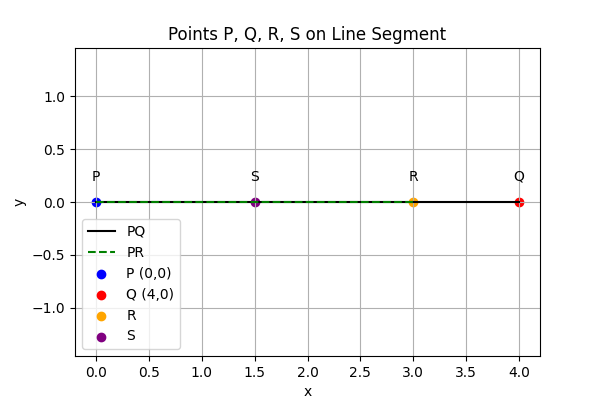
\includegraphics[width=0.75\columnwidth]{figs/graph.png}
\end{center}
\caption{}
\label{fig:Fig}
\end{figure}



\end{document}